\begin{wrapfigure}[0]{r}[0cm]{3cm}
 \vspace{-6cm}
 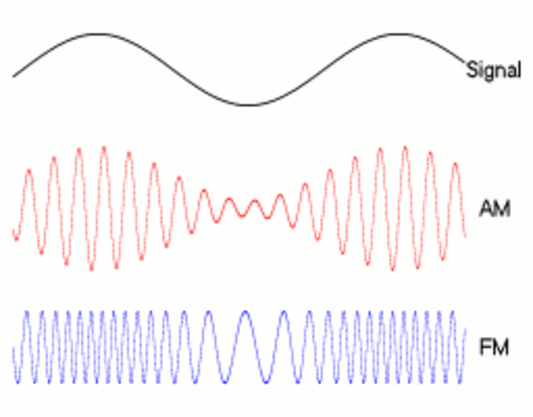
\includegraphics[scale=0.4]{Modulation/Bilder/Amfm3-en-de.pdf}
 \vspace{-6cm}
\end{wrapfigure}

\section*{Theorie- und Prüfungsfragen} 

\mucho{1}{TE106}
{Die Übermodulation eines SSB-Signals führt wahrscheinlich zu}%Frage
{verminderten Seitenbändern.}%A
{Kreuzmodulation.}%B
{ausgeprägten Splatter-Erscheinungen.}%C
{überhöhtem Hub.}%D
{C}%Lösung

\mucho{2}{TF317}
{Bei der Schaltung handelt es sich um einen\\ 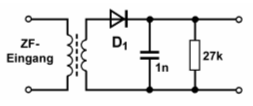
\includegraphics[scale=0.6]{Modulation/Bilder/TF318.png}}%Frage
{FM-Diskriminator.}%A
{AM-Detektor.}%B
{ZF-Modulator.}%C
{AGC-Gleichrichter.}%D
{B}%Lösung


\mucho{3}{TG301}
{Was kann man bezüglich der Ausgangsleistung eines FM-Senders in Abhängigkeit von der Modulation aussagen?}%Frage
{Sie reduziert sich um 50 $\%$, wenn der Sender moduliert wird.
}%A
{Sie variiert mit der Modulationsleistung, wenn der Sender moduliert wird.}%B
{Sie ist unabhängig von der Modulation.}%C
{Sie geht gegen Null, wenn der Sender nicht moduliert wird.}%D
{C}%Lösung

\mucho{4}{TD505}
{Bei dieser Schaltung handelt es sich um einen \\ 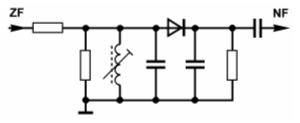
\includegraphics[scale=0.5]{Modulation/Bilder/TD505.png}}%Frage
{Flanken-Diskriminator zur Demodulation von FM-Signalen.}%A
{Produktdetektor zur Demodulation von SSB-Signalen.}%B
{Ratiodetektor zur Demodulation von FM-Signalen.}%C
{Synchrondemodulator zur Demodulation von AM-Signalen.}%D
{A}%Lösung

\mucho{5}{TD506}
{Bei dieser Schaltung handelt es sich um einen \\ 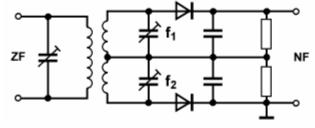
\includegraphics[scale=0.6]{Modulation/Bilder/TD506.png}}%Frage
{Gegentakt-Flanken-Diskriminator zur Demodulation von FM-Signalen.}%A
{Ratiodetektor zur Demodulation von FM-Signalen.}%B
{Hüllkurvendemodulator zur Demodulation von AM-Signalen.}%C
{Produktdetektor zu Demodulation von SSB-Signalen.}%D
{A}%Lösung

\mucho{6}{TD507}
{Bei dieser Schaltung handelt es sich um einen \\ 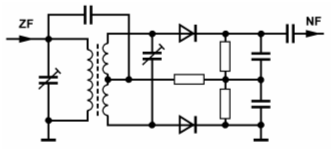
\includegraphics[scale=0.5]{Modulation/Bilder/TD507.png}}%Frage
{Produktdetektor zu Demodulation von SSB-Signalen.}%A
{Flanken-Diskriminator zur Demodulation von FM-Signalen.}%B
{Hüllkurvendemodulator zur Demodulation von AM-Signalen.}%C
{Phasendiskriminator zur Demodulation von FM-Signalen.}%D
{D}%Lösung

\mucho{7}{TD508}
{Bei dieser Schaltung handelt es sich um einen \\ 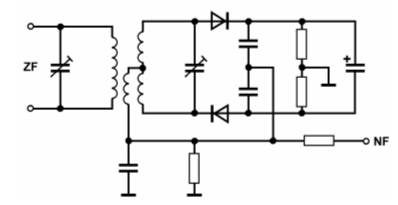
\includegraphics[scale=0.5]{Modulation/Bilder/TD508.png}}%Frage
{Flanken-Diskriminator zur Demodulation von FM-Signalen.}%A
{Hüllkurvendemodulator zur Demodulation von AM-Signalen.}%B
{Produktdetektor zur Demodulation von SSB-Signalen.}%C
{Ratiodetektor zur Demodulation von FM-Signalen.}%D
{D}%Lösung

\mucho{8}{TD509}
{Bei dieser Schaltung handelt es sich um einen \\ 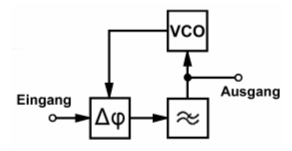
\includegraphics[scale=0.5]{Modulation/Bilder/TD509.png}}%Frage
{AM-Modulator.}%A
{SSB-Demodulator mit PLL-gesteuertem BFO.}%B
{PLL-FM-Demodulator.}%C
{ZF-Verstärker.}%D
{C}%Lösung
